%%
%% Automatically generated file from DocOnce source
%% (https://github.com/hplgit/doconce/)
%%
%%
% #ifdef PTEX2TEX_EXPLANATION
%%
%% The file follows the ptex2tex extended LaTeX format, see
%% ptex2tex: http://code.google.com/p/ptex2tex/
%%
%% Run
%%      ptex2tex myfile
%% or
%%      doconce ptex2tex myfile
%%
%% to turn myfile.p.tex into an ordinary LaTeX file myfile.tex.
%% (The ptex2tex program: http://code.google.com/p/ptex2tex)
%% Many preprocess options can be added to ptex2tex or doconce ptex2tex
%%
%%      ptex2tex -DMINTED myfile
%%      doconce ptex2tex myfile envir=minted
%%
%% ptex2tex will typeset code environments according to a global or local
%% .ptex2tex.cfg configure file. doconce ptex2tex will typeset code
%% according to options on the command line (just type doconce ptex2tex to
%% see examples). If doconce ptex2tex has envir=minted, it enables the
%% minted style without needing -DMINTED.
% #endif

% #define PREAMBLE

% #ifdef PREAMBLE
%-------------------- begin preamble ----------------------

\documentclass[%
oneside,                 % oneside: electronic viewing, twoside: printing
final,                   % or draft (marks overfull hboxes, figures with paths)
10pt]{article}

\listfiles               % print all files needed to compile this document

\usepackage[a4paper]{geometry}

\usepackage{relsize,makeidx,color,setspace,amsmath,amsfonts}
\usepackage[table]{xcolor}
\usepackage{bm,microtype}

\usepackage[pdftex]{graphicx}

\usepackage{ptex2tex}
% #ifdef MINTED
\usepackage{minted}
\usemintedstyle{default}
% #endif
\usepackage{fancyvrb}

\usepackage[T1]{fontenc}
%\usepackage[latin1]{inputenc}
\usepackage{ucs}
\usepackage[utf8x]{inputenc}

% Set palatino as the default font family:
\usepackage[sc]{mathpazo}    % Palatino fonts
\linespread{1.05}            % Palatino needs extra line spread to look nice

\usepackage{lmodern}         % Latin Modern fonts derived from Computer Modern

% Hyperlinks in PDF:
\definecolor{linkcolor}{rgb}{0,0,0.4}
\usepackage{hyperref}
\hypersetup{
    breaklinks=true,
    colorlinks=true,
    linkcolor=linkcolor,
    urlcolor=linkcolor,
    citecolor=black,
    filecolor=black,
    %filecolor=blue,
    pdfmenubar=true,
    pdftoolbar=true,
    bookmarksdepth=3   % Uncomment (and tweak) for PDF bookmarks with more levels than the TOC
    }
%\hyperbaseurl{}   % hyperlinks are relative to this root

\setcounter{tocdepth}{2}  % number chapter, section, subsection

%\VerbatimFootnotes must come after hyperref and footmisc packages
\VerbatimFootnotes

% Tricks for having figures close to where they are defined:
% 1. define less restrictive rules for where to put figures
\setcounter{topnumber}{2}
\setcounter{bottomnumber}{2}
\setcounter{totalnumber}{4}
\renewcommand{\topfraction}{0.85}
\renewcommand{\bottomfraction}{0.85}
\renewcommand{\textfraction}{0.15}
\renewcommand{\floatpagefraction}{0.7}
% 2. ensure all figures are flushed before next section
\usepackage[section]{placeins}
% 3. enable begin{figure}[H] (often leads to ugly pagebreaks)
%\usepackage{float}\restylefloat{figure}

\usepackage[framemethod=TikZ]{mdframed}

% --- begin definitions of admonition environments ---

% Admonition style "mdfbox" is an oval colored box based on mdframed
% "notice" admon
\colorlet{mdfbox_notice_background}{gray!5}
\newmdenv[
  skipabove=15pt,
  skipbelow=15pt,
  outerlinewidth=0,
  backgroundcolor=mdfbox_notice_background,
  linecolor=black,
  linewidth=2pt,       % frame thickness
  frametitlebackgroundcolor=mdfbox_notice_background,
  frametitlerule=true,
  frametitlefont=\normalfont\bfseries,
  shadow=false,        % frame shadow?
  shadowsize=11pt,
  leftmargin=0,
  rightmargin=0,
  roundcorner=5,
  needspace=0pt,
]{notice_mdfboxmdframed}

\newenvironment{notice_mdfboxadmon}[1][]{
\begin{notice_mdfboxmdframed}[frametitle=#1]
}
{
\end{notice_mdfboxmdframed}
}

% Admonition style "mdfbox" is an oval colored box based on mdframed
% "summary" admon
\colorlet{mdfbox_summary_background}{gray!5}
\newmdenv[
  skipabove=15pt,
  skipbelow=15pt,
  outerlinewidth=0,
  backgroundcolor=mdfbox_summary_background,
  linecolor=black,
  linewidth=2pt,       % frame thickness
  frametitlebackgroundcolor=mdfbox_summary_background,
  frametitlerule=true,
  frametitlefont=\normalfont\bfseries,
  shadow=false,        % frame shadow?
  shadowsize=11pt,
  leftmargin=0,
  rightmargin=0,
  roundcorner=5,
  needspace=0pt,
]{summary_mdfboxmdframed}

\newenvironment{summary_mdfboxadmon}[1][]{
\begin{summary_mdfboxmdframed}[frametitle=#1]
}
{
\end{summary_mdfboxmdframed}
}

% Admonition style "mdfbox" is an oval colored box based on mdframed
% "warning" admon
\colorlet{mdfbox_warning_background}{gray!5}
\newmdenv[
  skipabove=15pt,
  skipbelow=15pt,
  outerlinewidth=0,
  backgroundcolor=mdfbox_warning_background,
  linecolor=black,
  linewidth=2pt,       % frame thickness
  frametitlebackgroundcolor=mdfbox_warning_background,
  frametitlerule=true,
  frametitlefont=\normalfont\bfseries,
  shadow=false,        % frame shadow?
  shadowsize=11pt,
  leftmargin=0,
  rightmargin=0,
  roundcorner=5,
  needspace=0pt,
]{warning_mdfboxmdframed}

\newenvironment{warning_mdfboxadmon}[1][]{
\begin{warning_mdfboxmdframed}[frametitle=#1]
}
{
\end{warning_mdfboxmdframed}
}

% Admonition style "mdfbox" is an oval colored box based on mdframed
% "question" admon
\colorlet{mdfbox_question_background}{gray!5}
\newmdenv[
  skipabove=15pt,
  skipbelow=15pt,
  outerlinewidth=0,
  backgroundcolor=mdfbox_question_background,
  linecolor=black,
  linewidth=2pt,       % frame thickness
  frametitlebackgroundcolor=mdfbox_question_background,
  frametitlerule=true,
  frametitlefont=\normalfont\bfseries,
  shadow=false,        % frame shadow?
  shadowsize=11pt,
  leftmargin=0,
  rightmargin=0,
  roundcorner=5,
  needspace=0pt,
]{question_mdfboxmdframed}

\newenvironment{question_mdfboxadmon}[1][]{
\begin{question_mdfboxmdframed}[frametitle=#1]
}
{
\end{question_mdfboxmdframed}
}

% Admonition style "mdfbox" is an oval colored box based on mdframed
% "block" admon
\colorlet{mdfbox_block_background}{gray!5}
\newmdenv[
  skipabove=15pt,
  skipbelow=15pt,
  outerlinewidth=0,
  backgroundcolor=mdfbox_block_background,
  linecolor=black,
  linewidth=2pt,       % frame thickness
  frametitlebackgroundcolor=mdfbox_block_background,
  frametitlerule=true,
  frametitlefont=\normalfont\bfseries,
  shadow=false,        % frame shadow?
  shadowsize=11pt,
  leftmargin=0,
  rightmargin=0,
  roundcorner=5,
  needspace=0pt,
]{block_mdfboxmdframed}

\newenvironment{block_mdfboxadmon}[1][]{
\begin{block_mdfboxmdframed}[frametitle=#1]
}
{
\end{block_mdfboxmdframed}
}

% --- end of definitions of admonition environments ---

% prevent orhpans and widows
\clubpenalty = 10000
\widowpenalty = 10000

% --- end of standard preamble for documents ---


% insert custom LaTeX commands...

\raggedbottom
\makeindex

%-------------------- end preamble ----------------------

\begin{document}

% endif for #ifdef PREAMBLE
% #endif


% ------------------- main content ----------------------



% ----------------- title -------------------------

\thispagestyle{empty}

\begin{center}
{\LARGE\bf
\begin{spacing}{1.25}
Liten JavaScript kurs rettet mot IT2
\end{spacing}
}
\end{center}

% ----------------- author(s) -------------------------

\begin{center}
{\bf Johan Hake${}^{}$ (\texttt{johan.hake@gmail.com})} \\ [0mm]
\end{center}

\begin{center}
% List of all institutions:
\end{center}
    
% ----------------- end author(s) -------------------------

\begin{center} % date
Aug 10, 2015
\end{center}

\vspace{1cm}


% sphinx code-blocks: js=javascript pycod=python cod=fortran cppcod=c++ sys=console



% inline figure
\centerline{
\includegraphics[width=0.5\linewidth]{figures/javascript-seeklogo.pdf}}




\pagebreak

\section{Forord}
\label{section:forord}

Dette er en ressurs for elever og lærere som ønsker å bruke
javascript/HTML/CSS som programmeringsspråk i IT2-undervisningen. Hele
nettstedet/boka har betastatus, og innhold vil fylles på og endres
fortløpende. Dokumentet er basert på en WordPress
\href{{http://www.fuzzbin.org/IT2}}{\nolinkurl{versjon}} utarbeidet av Tom Jarle
Christiansen. Han har også lagd de fleste av kodeeksemplene og youtube
filmene. Et stort takk rettes derfor til Tom Jarle!

Dokumentet er bygget opp etter strukturen til kompetansemåla i faget,
(se avsnitt:~\ref{section:kompetansemål}), og inneholder teori,
oppgaver og videoer. Relevante kodeeksempler finnes på
\href{{http://gist.github.com/johanhake}}{`gist.github'} og jsBin. Du kan
også laste ner alle kode eksemplene og oppgavene
\href{{https://github.com/johanhake/it2/blob/master/kode.zip?raw=true}}{\nolinkurl{her}}.

Dokumentet er lagd med hjelp
\href{{http://hplgit.github.io/doconce/doc/web/index.html}}{\nolinkurl{doconce}}.  Et
stort takk rettes til visjonæren Hans Petter
\href{{http://hplgit.github.io/homepage/index.html}}{\nolinkurl{Langtangen}} som har
utarbeidet dette verktøy.

% Bli gjerne med i nettverket for lærere som er interessert i IT2 med
% javascript på \href{{https://www.facebook.com/groups/231993360276497}}{\nolinkurl{facebook}}.

Du står helt fritt til å bruke innholdet du finner i dette dokumentet
slik du selv måtte ønske, så lenge du deler videre med vilkårene
under. 

\href{{mailto:johan.hake@gmail.com}}{\nolinkurl{Johan Hake}}, August 2015

Dette verk er lisensieret under en Creative Commons
Navngivelse-DelPåSammeVilkår 3.0 Norge
\href{{http://creativecommons.org/licenses/by-sa/3.0/no/}}{\nolinkurl{lisens}}.

% !split

\pagebreak

\section{Teori}

Den grunnleggende teorin i faget er delt opp i avsnitt som tilsvarer
kompetansemålene i faget:

\begin{itemize}
\item Multimedieutvikling, se avsnitt~\ref{section:teori:multimedieutvikling}

\item Programmering, se avsnitt~\ref{section:teori:programmering}

\item Planlegging og dokumentasjon, se avsnitt~\ref{section:teori:planlegging}
\end{itemize}

\noindent
% !split

\subsection{Multimedieutvikling}
\label{section:teori:multimedieutvikling}

\paragraph{Editor og filbehandling.}
\label{section:teori:editorogfilbehandling}

Gode verktøy er helt avgjørende uansett hva slags jobb vi skal
gjøre. Dette gjelder også når vi skal programmere. I denne boka
skal vi benytte oss av to typer verktøy.

\begin{description}
\item[Nettleser:] 
  Program der koden kjøres og skjermbildet vises

\item[Editor:] 
  Her skrives og editeres programkoden 
\end{description}

\noindent
\paragraph{Nettlesere.}

De fleste moderne nettlesere fungerer veldig bra som støtteverktøy
til programmering. De har de funksjoner og verktøy som trengs for å
jobbe med HTML-programmering på en effektiv og god måte. De mest
brukte nettleserne i dag er Chrome, FireFox, Internet Explorer, Opera
og Safari.

\paragraph{Editor.}

Det finnes veldig mange gode editorer for programmering. De mest
avanserte er store programmeringsmijø, eller
\href{{http://en.wikipedia.org/wiki/Integrated_development_environment}}{\nolinkurl{IDE'er}}
som de også kalles. I dette kurset kommer vi langt med noe enklere
editorer, som allikevel er veldig kraftige og funksjonsrike.


\begin{figure}[t]
  \centerline{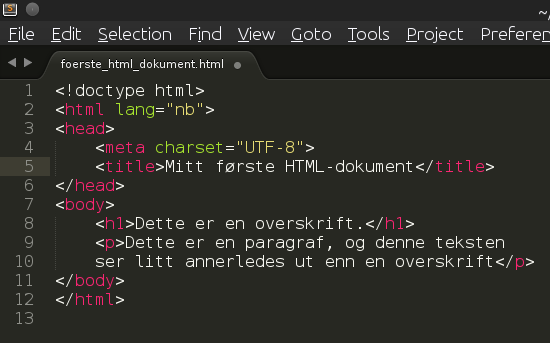
\includegraphics[width=0.5\linewidth]{figures/editor_sublime_eksempel.png}}
  \caption{
  Et lite ekesmpel på hvordan et enkelt HTML-dokument kan se ut.
  }
\end{figure}
%\clearpage % flush figures 


Til dette kurset anbefaler jeg at dere bruker
\href{{https://notepad-plus-plus.org}}{\nolinkurl{notepad++}} eller \href{{http://www.sublimetext.com/2}}{\nolinkurl{Sublime
Text}} 2. Disse er enkle, men allikevel
kraftige kodeeditorer der man enkelt og oversiktlig kan jobbe med
flere filer samtidig. De har også god støtte for automatiske
kodeforslag og fargelegging av kode slik at lesing går lettere.

\paragraph{Før vi lager vårt første html-side.}

Nå er vi straks klare til å sette i gang med det som er gøy, men
før det må vi ha noen få ting på plass...


\begin{notice_mdfboxadmon}[Før vi lager vårt første html-side må vi...]
\begin{enumerate}
\item Lag en mappe som skal inneholde filene du lager. (Hvert program skal ha sin egen mappe).

\item Lag et nytt html-dokument som inneholder koden under. (Se under for startkoder).
\end{enumerate}

\noindent
\end{notice_mdfboxadmon}



\paragraph{Example: Kom igang med editorn.}
\label{example:komigang}


\begin{notice_mdfboxadmon}[Programkoden som du kan bruke i et HTML-dokument for å komme i gang.]
\bhtml
<!doctype html>
<html lang="nb">
<head>
	<meta charset="UTF-8">
	<title>Mitt første HTML-dokument</title>
</head>
<body>
	<h1>Dette er en overskrift.</h1> 
	<p>Dette er en paragraf, og denne teksten ser litt annerledes 
          ut enn en overskrift</p>
</body>
</html>

\ehtml
\end{notice_mdfboxadmon}

 

% !split

\paragraph{HTML.}
\label{section:teori:html} 

\textbf{HyperText Markup Language} (HTML, hypertekstmarkeringsspråk) er et
\href{{http://no.wikipedia.org/wiki/Markeringsspråk}}{\nolinkurl{markeringsspråk}} for
formatering av \href{{http://no.wikipedia.org/wiki/Nettside}}{\nolinkurl{nettsider}}
med \href{{http://no.wikipedia.org/wiki/Hypertekst}}{`hypertekst'} og annen
informasjon som kan vises i en
\href{{http://no.wikipedia.org/wiki/Nettleser}}{\nolinkurl{nettleser}}. HTML benyttes
til å strukturere informasjon - angi noe tekst som overskrifter,
avsnitt, lister og så videre - og kan, i en viss grad, brukes til å
beskrive utseende og semantikk i et dokument.

HTML ble opprinnelig definert i 1989 av \href{{https://no.wikipedia.org/wiki/Tim_Berners-Lee}}{\nolinkurl{Tim
Berners-Lee}} og
\href{{https://en.wikipedia.org/wiki/Robert_Cailliau}}{\nolinkurl{Robert Caillau}} og
videreutviklet av \href{{http://no.wikipedia.org/wiki/IETF}}{\nolinkurl{IETF}} og er
nå en internasjonal standard
(\href{{http://no.wikipedia.org/wiki/International_Organization_for_Standardization}}{\nolinkurl{ISO}}/\href{{http://no.wikipedia.org/wiki/International_Electrotechnical_Commission}}{\nolinkurl{IEC}}
15445:2000). Siden har HTML-spesifikasjonene blitt opprettholdt av
\href{{http://no.wikipedia.org/wiki/World_Wide_Web_Consortium}}{\nolinkurl{World Wide Web
Consortium}}
(W3C)\footnote{Hentet fra wikipediaartikkelen om \href{{http://no.wikipedia.org/wiki/HTML}}{\nolinkurl{HTML}}.}. 



\paragraph{Programmering i HTML.}

Et HTML-dokument består av koder, eller "tagger" som beskriver hvordan
vi vil at siden skal se ut, og i noen grad hva slags funksjonalitet
den skal ha. I tabellen under finner du noen av de vanligste kodene
som brukes\footnote{For en utfyllende liste se \href{{http://www.w3schools.com/tags/ref_byfunc.asp}}{\nolinkurl{http://www.w3schools.com}}.}.




\providecommand{\specialcell}[2][c]{\begin{tabular}[c]{@{}#1@{}}#2\end{tabular}}
{\footnotesize\renewcommand{\arraystretch}{1.2}
\vspace{2em}
\begin{tabular}{|l|l|l|}
\hline
\textbf{Tag} & \textbf{Beskrivelse} & \textbf{Eksempel på bruk}\\
\hline
\texttt{<h1>...<h6>} & Overskrift & \texttt{<h3>Dette er en liten overskrift</h3>}\\
\hline
\texttt{<p>} & Avsnitstekst & \texttt{<p>Denne teksten blir samlet i et avsnitt.</p>}\\
\hline
\texttt{<b>} & Fet skrift & \texttt{<b>Denne teksten blir fet</b>}\\
\hline
\texttt{<i>} & Kursiv & \texttt{<i>Denne teksten er i kursiv</i>}\\
\hline
\texttt{<br>} & Linjeskift & \specialcell[l]{\texttt{Tekst på en linje<br>}\\\texttt{Tekst på linja under}}\\
\hline
\texttt{<hr>} & Horisontal linje & \texttt{<hr>}\\
\hline
\texttt{<a>} & Hyperlenke & \specialcell[l]{\texttt{<a href="http://www.w3c.org">}\\\texttt{Fagnettsted</a>}}\\
\hline
\texttt{<a>} & Epostlenke & \specialcell[l]{\texttt{<a href="mailto:postmottak@kd.dep.no">}\\\texttt{Send e-post</a>}}\\
\hline
\texttt{<img>} & Sette inn bilde & \texttt{<img src="mittBilde.jpg">}\\
\hline
\texttt{<ul> og <li>} & Punktliste & \specialcell[l]{\texttt{<ul>}\\\texttt{  <li>Punkt 1</li>}\\\texttt{  <li>Punkt 2</li>}\\\texttt{</ul>}}\\
\hline
\texttt{<ol> og <li>} & Nummerert liste & \specialcell[l]{\texttt{<ol>}\\\texttt{  <li>Punkt 1</li>}\\\texttt{  <li>Punkt 2</li>}\\\texttt{</ol>}}\\
\hline
\specialcell[l]{\texttt{<table>, <tr>}\\\texttt{og <td>}} & Tabell & \specialcell[l]{\texttt{<table>}\\\texttt{  <tr><td>Celle1</td><td>Celle2</tr>}\\\texttt{  <tr><td>Celle1</td><td>Celle2</tr>}\\\texttt{</table>}}\\
\hline
\end{tabular}
}\renewcommand{\arraystretch}{1.0}
\\


Fra tabellen ser vi at noen tagger trenger en lukketag, som sier nåt
taggen slutter, f eks: \texttt{</a>}, \texttt{</tr>} og \texttt{</td>}. Hvis ikke en
lukketag følger den tilsvarende åpningstaggen får vi et syntaksfeil og
siden kan oftest ikke vises. Noen tagger trenger ikke en lukketag, f
eks: \texttt{<hr>} og \texttt{<br>}.

HTML-koden settes sammen i et HTML-dokument som igjen kan vises i en
nettleser.


\begin{block_mdfboxadmon}[]
\bhtml
<!doctype html>
<html lang="nb">
<head>
	<meta charset="UTF-8">
	<title>Mitt første HTML-dokument</title>
</head>
<body>
	<h1>Dette er en overskrift.</h1> 
	<p>Dette er en paragraf, og denne teksten ser litt annerledes 
          ut enn en overskrift</p>
</body>
</html>
\ehtml
\end{block_mdfboxadmon}



Hvert html dokument må ha noen standard tagger som \Verb?<!doctype>? og
\texttt{<html>}. \href{{http://www.w3schools.com/tags/tag_doctype.asp}}{\nolinkurl{doctype}}
taggen sier til en netleser at det er et html dokument og
\href{{http://www.w3schools.com/tags/tag_html.asp}}{\nolinkurl{html}} taggen sier hvor
selve html koden kommer. Vi ser fra eksempelet at \texttt{<html>} taggen har
en så kallt attributt: \texttt{lang="no"}, som er tileggsinformasjon til
taggen, se nedan. På rad 3-6 defineres \texttt{<head>}
\href{{http://www.w3schools.com/tags/tag_head.asp}}{\nolinkurl{taggen}}, som bestemmer
egenskaper til hele html siden, for eksempel titel og tegnsett
(encoding). En html dokument bør også ha en \texttt{<body>} tag. Denne
\href{{http://www.w3schools.com/tags/tag_body.asp}}{\nolinkurl{taggen}} inneholder det
som skall vises på siden.

\paragraph{Example: Test tagger.}
\label{example:testtagger}


\begin{notice_mdfboxadmon}[Test ulike tagger gjennom å laste in filen i en editor og en nettleser]
\bhtml
<!DOCTYPE html>
<html>
<head>
    <meta charset="utf-8">
    <title>Tagtesting!</title>
</head>
<body>
    <h1>Test tagger her!</h1>
    <p>Prøv deg selv med egen kode ved å skrive i HTML-fanen.</p>
</body>
</html>
\ehtml
\end{notice_mdfboxadmon}

 

\paragraph{Attributter.}

Attributter brukes for å gi ekstra informasjon til hva taggen skal
gjøre. En attributt plasseres inne i taggen, og kan for eksempel
inneholde informasjon om bakgrunnsfarge, plassering eller
identifikatorer som skal gjelde for den aktuelle taggen. Det er fullt
mulig å ha flere attributter i samme tag.


\providecommand{\specialcell}[2][c]{\begin{tabular}[c]{@{}#1@{}}#2\end{tabular}}
{\footnotesize\renewcommand{\arraystretch}{1.2}
\vspace{2em}
\begin{tabular}{|l|l|l|}
\hline
\textbf{Attributtnavn} & \textbf{Egenskap} & \textbf{Eksempel}\\
\hline
\texttt{align} & Plassering av teksten & \specialcell[l]{\texttt{<h1 align="right">Denne}\\\texttt{overskriften vil stå på høyre side</h1>}}\\
\hline
\texttt{bgcolor} & Bakgrunnsfarge & \specialcell[l]{\texttt{<h1 bgcolor="green">Denne}\\\texttt{overskriften vil ha grønn bakgrunn</h1>}}\\
\hline
\texttt{height og width} & \specialcell[l]{Høyde og bredde på bilder,\\tabeller og celler} & \texttt{<table width="300px">}\\
\hline
\end{tabular}
}\renewcommand{\arraystretch}{1.0}
\\


Attributter er en viktig del av et HTML-dokument, og gjør at vi kan
\emph{finjustere} taggene til å vise innhold slik vi ønsker. For mer
avansert design og utseende må vi benytte oss av CSS.


\begin{notice_mdfboxadmon}[Her brukes attributtene src og width for å gi egenskaper til bilde-taggen]
\bhtml
<body>
  <h1>Min timeplan</h1>
  <img src="bilder/klasserom.jpg" width="400px">
</body>
\ehtml
\end{notice_mdfboxadmon}



\paragraph{input.}

Veldig ofte ønsker vi at brukeren skal legge inn informasjon slik at
den kan lagres eller bearbeides. For å få til dette kan vi bruke
\texttt{<input>}. Ved å bruke denne taggen sammen med ulike attributter kan vi
lage elementer som tekstbokser, radioknapper, draknapper, datobokser
osv. \texttt{<input>} brukes ofte sammen med \texttt{<form>} som samler alle
input-tagger i et skjema. Selv om \texttt{<input>} kun er en enkelt tag, så
kan man få den til å ha mange former ved å bruke attributten \texttt{type}.


\begin{notice_mdfboxadmon}[Eksempel på input-tag]
\bhtml
<form>
Fornavn: <input type="text"><br>
Etternavn: <input type="text">
</form>
\ehtml
\end{notice_mdfboxadmon}



Det finnes mange ulike typer inputfelt. I tabellen under finner du
eksempel på flere.


\providecommand{\specialcell}[2][c]{\begin{tabular}[c]{@{}#1@{}}#2\end{tabular}}
{\footnotesize\renewcommand{\arraystretch}{1.2}
\vspace{2em}
\begin{tabular}{|l|l|}
\hline
\textbf{Type} & \textbf{Beskrivelse}\\
\hline
button & Vanlig trykknapp\\
\hline
color & Fargevelger\\
\hline
date & Datovelger\\
\hline
datetime & Dato- og tidsvelger\\
\hline
email & Tekstfelt for epost\\
\hline
month & Månedsvelger\\
\hline
password & Tekstfelt for passord\\
\hline
radio & Radioknapper\\
\hline
range & Glideknapp\\
\hline
reset & Nulstiller alt som er inne i samme form\\
\hline
search & Søkefelt\\
\hline
submit & Sender all data som er i samme form\\
\hline
tel & Felt for telefonnummer\\
\hline
text & Tekstfelt\\
\hline
time & Klokkeslett\\
\hline
url & Felt for nettadresser\\
\hline
week & Ukevelger\\
\hline
checkbox & Avkryssingsbokser\\
\hline
number & Tallvelger\\
\hline
\end{tabular}
}\renewcommand{\arraystretch}{1.0}
\\


\paragraph{Example: Test input.}
\label{example:testinput}


\begin{notice_mdfboxadmon}[Test ulike input-typer gjennom å laste in filen i en editor og en nettleser]
\bhtml
<!DOCTYPE html>
<html>
<head>
    <meta charset="utf-8">
    <title>JS Bin</title>
</head>
<body>
    <h1> Her kan du teste ulike input-typer</h1><br>
    <p>Prøv for eksempel: "color", "checkbox" eller "number".
    <input type="text">
</html>
\ehtml
\end{notice_mdfboxadmon}

 

\paragraph{taggene video og audio.}


\href{{http://www.w3schools.com/tags/tag_video.asp}}{\nolinkurl{Video}} og
\href{{http://www.w3schools.com/tags/tag_audio.asp}}{\nolinkurl{audio}}-taggene er
brukes når man skal spille av film og lyd. Flere formater støttes, og
man har mulighet for volum og avspillingskontroll.


\begin{notice_mdfboxadmon}[Eksempel på audio og video-tagger med ulike attributter]
\bhtml
<audio controls>
    <source src="lyd.ogg">
</audio>
<video width="320" height="240" controls>
  <source src="film.ogg">
</video>
\ehtml
\end{notice_mdfboxadmon}

 

\paragraph{div.}

\texttt{<div>} er en fin måte å lage et avgrenset område på
nettsiden. \texttt{<div>} i seg selv er kun et tomt skall, og vi er nødt til
å fylle på med innhold mellom start- og slut-taggen. Ved å bruke
attributter på div-taggen kan vi få den til å se ut på mange
forskjellige måter.

\paragraph{Example: Lek med div.}
\label{example:Lekmeddiv}


\begin{notice_mdfboxadmon}[Her kan du endre på div-style attributten selv gjennom å laste in filen i en editor og en nettleser]


% inline figure
\centerline{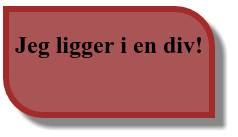
\includegraphics[width=0.5\linewidth]{figures/jeg_ligger_i_en_div.png}}



\bhtml
<!DOCTYPE html>
<html>
<head>
  <meta charset="utf-8">
  <title>Leke med div</title>
</head>
<body>
	<div  style="text-align: center;
            width: 200px;
            height: 100px;
            background-color: #aa5555;
            border-color: brown;
            border-width: 6px;
            border-style: solid;
            border-radius: 0px 40px;
            box-shadow: 10px 10px 5px #888888;">
      <h2>Jeg ligger i en div!</h2></div>
</body>
</html>
\ehtml
\end{notice_mdfboxadmon}

 

Det finnes så mange html-tagger og ulike attributter at de færreste
husker alle selv. Det er derfor viktig å lære seg å slå
opp. \href{{http://W3schools.com}}{\nolinkurl{W3schools.com}} er et nettsted der du
selv kan finne tagger, og se eksempler på hvordan de brukes.

\paragraph{DOM treet.}

Når en webside lastes skaper nettleseren en Document Object Model
(DOM) av siden. HTML DOM modellen skapes som et tre av objekter, se
figur~\ref{figure:domtree}. DOM er en W3C standard, som definerer
metoder for å få tilgang på og endre et HTML (eller XML) dokument.


\begin{figure}[t]
  \centerline{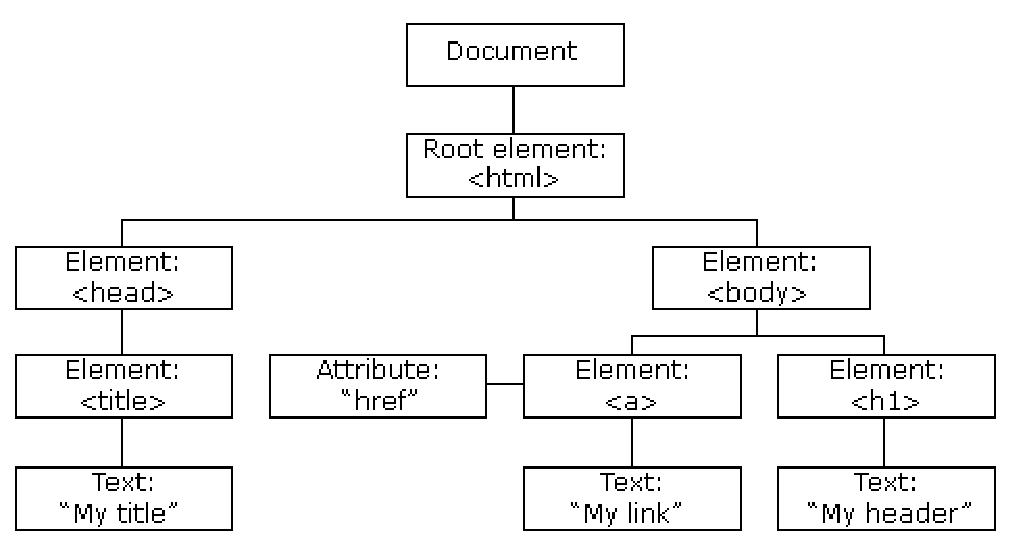
\includegraphics[width=0.9\linewidth]{figures/pic_htmltree.pdf}}
  \caption{
  Et HTML DOM tre av objekter (hentet fra \href{{http://www.w3schools.com/js/js_htmldom.asp}}{\protect `www.w3schools.com`}). \label{figure:domtree}
  }
\end{figure}
%\clearpage % flush figures figure:domtree


% When a web page is loaded, the browser creates a Document Object Model
% of the page.  The HTML DOM model is constructed as a tree of Objects:

% !split

\paragraph{CSS.}
\label{section:teori:css} 

% !split

\subsection{Programmering}
\label{section:teori:programmering}

% !split
\subsection{Planlegging og dokumentasjon}
\label{section:teori:planlegging}

% !split

\pagebreak

\section{Læreplan i informasjonsteknologi}

Dette avsnittet er hentet fra \href{{http://www.udir.no/kl06/inf1-01/Hele}}{\nolinkurl{udir}}.

\subsection{Formål}

Informasjonsteknologien har hatt stor betydning for
samfunnsutviklingen de siste tiårene. Teknologien har i løpet av kort
tid endret kommunikasjonsmønsteret i samfunnet og skapt nye
arbeidsplasser og lærings- og forskningsarenaer. Samfunnet har behov
for mennesker som kan forstå, benytte og videreutvikle
informasjonsteknologien, men samfunnet trenger også mennesker med en
bevisst og kritisk holdning til hva teknologien gjør med mennesker og
samfunn. Informasjonsteknologien gir muligheter for å lage helt nye
produkter og tjenester gjennom kreativitet og samarbeid over
faggrenser, og bidrar dermed til teknologisk innovasjon.

Programfaget skal gi trening i kreativ tenkning og problemløsning og
i å formulere presise beskrivelser og finne generelle
mønstre. Programfaget skal bidra til å gi innsikt i hvordan
informasjon i form av tall, tekster, bilder, grafikk, film, lyd og
animasjoner kan struktureres og behandles automatisk som data, og
hvilke krav det setter til datamaskiner og annet digitalt
utstyr. Gjennom programfaget skal den enkelte få erfaring med bruk av
moderne teknologi og relevante utviklingsverktøy, og hvordan
sammensmelting av data-, lyd- og bildeteknologi kan gi rom for
skapende bruk av teknologien.

Opplæringen legger vekt på å konstruere IT-løsninger, og
informasjonsteknologi er derfor på mange måter et praktisk fag. Det
skal legges til rette for kommunikasjon og samarbeid i
programfaget. Programfaget informasjonsteknologi er et realfag, men
det har også sterke koblinger til mediefag, samfunnsfag, økonomi,
språkfag og formgivingsfag. Programfaget kan derfor gi et godt
grunnlag for studier innen ulike fagområder og for videreutvikling av
kompetanse i yrkeslivet.

\subsection{Grunnleggende ferdigheter}

Grunnleggende ferdigheter er integrert i kompetansemålene der hvor de
bidrar til utvikling av og er en del av fagkompetansen. I
informasjonsteknologi forstås grunnleggende ferdigheter slik:


\begin{block_mdfboxadmon}[]

\textbf{Å kunne uttrykke seg muntlig og skriftlig} i informasjonsteknologi
innebærer å planlegge og beskrive IT-løsninger, og utarbeide
brukerveiledninger og dokumentasjon. Videre vil det si å formulere
presise instruksjoner for datamaskiner i et programmeringsspråk. Det
betyr også å uttrykke seg på en klar og presis måte.

\textbf{Å kunne lese} i informasjonsteknologi innerærer å tolke beskrivelser,
brukerveiledninger, diagrammer, modeller, symboler og programkode på
en presis måte. Videre betyr det å forstå fagspesifikke tekster.

\textbf{Å kunne regne} i informasjonsteknologi innebærer å gjøre enkle
utregninger eller uttrykke formler i et programmeringsspråk. Videre
vil det si å bruke enkel matematisk logikk for å uttrykke en
betingelse på en presis måte.

\textbf{Å kunne bruke digitale verktøy} utgjør en grunnstamme i
informasjonsteknologi. Det innebærer å bruke IT-løsninger på en
effektiv måte og bruke digitale verktøy både i planleggings- og
dokumentasjonsprosesser.
\end{block_mdfboxadmon}



\subsection{Kompetansemål IT2}
\label{section:kompetansemål}

\paragraph{Planlegging og dokumentasjon.}
Hovedområdet handler om planlegging av IT-løsninger, og utvikling av
disse etter gitte spesifikasjoner for å oppfylle brukernes
behov. Videre dreier det seg om dokumentasjon og vurdering av
IT-løsninger. Hovedområdet omfatter også utforming, dokumentasjon og
vurdering av løsninger i forhold til retningslinjer for
brukergrensesnitt.


\begin{notice_mdfboxadmon}[Mål for opplæringen er at eleven skal kunne:]
\begin{enumerate}
\item spesifisere og begrunne funksjonelle krav til planlagte IT-løsninger 

\item velge og bruke relevante teknikker og verktøy for planlegging og utvikling av IT-løsninger

\item lage brukerveiledninger for IT-løsninger

\item gjøre rede for hvordan IT-løsninger utvikles i samarbeid mellom personer, og hvilke krav det setter til planleggings- og utviklingsprosessen

\item forklare hensikten med teknisk dokumentasjon og lage slik dokumentasjon for IT-løsninger, med spesiell vekt på å dokumentere grensesnitt mellom ulike delsystemer
\end{enumerate}

\noindent
\end{notice_mdfboxadmon}



\paragraph{Programmering.}
Hovedområdet handler om hvordan formelle språk kan brukes til å
formulere strukturer og sette sammen instruksjoner som kan utføres av
en datamaskin. Sentralt i hovedområdet er eksperimentering og
problemløsning. I tillegg dreier det seg om objektorientering.


\begin{notice_mdfboxadmon}[Mål for opplæringen er at eleven skal kunne:]
\begin{enumerate}
\item lese og bruke dokumentasjon og kode

\item definere variabler og velge hensiktsmessige datatyper

\item tilordne uttrykk til variabler

\item programmere med enkle og indekserte variabler eller andre kolleksjoner av variabler

\item programmere med valg og gjentakelser

\item lage egne og bruke egne og andres funksjoner eller metoder med parametere

\item programmere funksjoner eller metoder som blir aktivisert av hendelser

\item utvikle og sette sammen delprogrammer

\item teste og finne feil i programmer ved å bruke vanlige teknikker

\item gjøre rede for hensikten med objektorientert utvikling og begrepene klasse, objekt og arv
\end{enumerate}

\noindent
\end{notice_mdfboxadmon}

 

\paragraph{Multimedieutvikling.}
Hovedområdet handler om utforming, strukturering, implementering og
vurdering av multimedieapplikasjoner med tall, tekst, lyd, bilde,
video og animasjoner. I tillegg omfatter hovedområdet både
applikasjoner for lokal bruk og publisering over Internett.


\begin{notice_mdfboxadmon}[Mål for opplæringen er at elevene skal kunne:]
\begin{enumerate}
\item planlegge og utvikle multimedieapplikasjoner ved å kombinere egne og andres multimedieelementer av typene tekst, bilde, lyd, video og animasjoner

\item bruke programmeringsspråk i multimedieapplikasjoner

\item vurdere og bruke relevante filformater for tekst, bilde, lyd, video og animasjoner

\item vurdere multimedieprodukter med hensyn til brukergrensesnitt og funksjonalitet
\end{enumerate}

\noindent
\end{notice_mdfboxadmon}

 

% !split


% ------------------- end of main content ---------------


% #ifdef PREAMBLE
\printindex

\end{document}
% #endif

